%% Algèbre
%\newcommand{\trans}[1]{#1^\top}  % transposé
%\newcommand{\dual}[1]{#1^\ast}  % dual
\newcommand{\clot}[1]{\bar{#1}}  % clôture algèbrique
\newcommand{\card}[1]{\# #1}  % cardinalité d'un ensemble
\newcommand{\LK}{\mathbb{L}}  % encore un corps
\newcommand{\U}{\mathbb{U}}  % encore un corps
\newcommand{\isom}{\cong}  % isomorphisme de corps
\newcommand{\frob}{\varphi}  % l'isomorphisme de frobenius
\newcommand{\res}{\rho}  % the residue form
\newcommand{\euler}{\phi}  % indicatrice d'Euler
\newcommand{\Cyclo}{\Phi}  % le polynome cyclotomique
%% Courbes
\newcommand{\Proj}{\mathbb{P}}  % espace projectif
\newcommand{\0}{\mathcal{O}}  % point de base d'une courbe
\newcommand{\ecpoint}[3]{[#1:#2:#3]}  % un point d'une courbe
\newcommand{\isog}[1]{\mathcal{#1}}  % la police des isogénies
\newcommand{\I}{\isog{I}}  % une isogénie I
\newcommand{\frobisog}{\phi}  % l'isogénie de frobenius
\newcommand{\Hasse}{H}  % l'invariant de Hasse
\newcommand{\divpol}{f}  % polynôme de division
%% Autre
\newcommand{\tildO}{\tilde{O}}  % la notation O~ qui oublie les log
\newcommand{\Mult}{\mathrm{\sf M}}  % fonction de multiplication
\newcommand{\ModComp}{\mathrm{\sf C}}  % fonction de composition modulaire
\newcommand{\alg}[1]{{\sf #1}}  % la police des algorithmes
\newcommand{\algref}[1]{\alg{\ref{#1}}}  % la police des algorithmes
\newcommand{\wrt}{\dashv}  % appartenance forte, a\wrt A signifie que a est représenté comme un élément de A
\newcommand{\ndiv}{\nmid}  % ne divise pas


\part{Calcul d'isogenies et applications cryptographiques}

%% these.tex
%% Copyright 2010 Luca De Feo
%% All rights reserved


Let $E$ and $E'$ be two elliptic curves defined over $\K$, by finding
an \emph{explicit isogeny} we mean to find a $\K$-rational function
from $E(\clot{\K})$ to $E'(\clot{\K})$ such that the map it defines is
an isogeny.

In this chapter we are interested in finding explicit isogenies of
ordinary elliptic curves over finite fields. In what follows $\F_q$
will be a finite field of characteristic $p$, and $d$ the positive
integer such that $q=p^d$.

\pdfmctwo{Given more details on "what's changed".}
Parts of this chapter and of the following have been published
in~\cite{df10}. However, the complexity analysis we give in
Proposition~\ref{th:lercier-sirvent} benefits from recent advances on
the computation of modular polynomials~\cite{sutherland10:modpol};
this in turn changes the relative ranking of the algorithms of this
chapter in terms of complexity. We also present a new algorithm in
Section~\ref{sec:bounded}.


\section{Overview}
\label{sec:history}

The problem of computing an explicit degree $\ell$ isogeny between two
given elliptic curves over $\F_q$ was originally motivated by point
counting methods based on Schoof's
algorithm~\cite{atkin88,elkies98,schoof95}. A review of the most
efficient algorithms to solve this problem is given
in~\cite{bostan+morain+salvy+schost08}, together with a new
quasi-optimal algorithm that we will review in Section~\ref{sec:bmss}.

All the algorithms of~\cite{bostan+morain+salvy+schost08} only work
when $\ell\ll p$. The case where $p$ is small compared to $\ell$ was
first treated by Couveignes in~\cite{couveignes94}, making use of
formal groups. The complexity of his method is $\tildO(\ell^3\log q)$ operations in
$\F_p$ assuming $p$ is constant, however it has an exponential
complexity in $\log p$.

Later, Lercier~\cite{lercier96} gave an algorithm specific to
characteristic $2$, that uses some linear properties of the problem to
build a linear system from whose solution the isogeny can be deduced.
Its complexity is conjectured to be $\tildO(\ell^3\log q)$ operations
in $\F_p$, but it has a much better constant factor
than~\cite{couveignes94}. At the moment we write, this is by many
orders of magnitude the fastest algorithm to solve practical instances
of the problem when $p=2$, thus being the \emph{de facto} standard for
cryptographic use.

Couveignes, again, proposed an algorithm in~\cite{couveignes96}
working for any $p$, based on the structure of the $p^k$ torsion of
ordinary elliptic curves. Using improvements
from~\cite{couveignes00,df+schost09,df10}, this algorithm has a
quadratic complexity in $\ell$. We review the original algorithm as
well as its improved variants in Sections~\ref{sec:C2}
to~\ref{sec:bounded}.

\pdfmcone{A little more crypto here.}
After the discovery of $p$-adic alternatives to Schoof's
algorithm~\cite{satoh00,fouquet+gaudry+harley00}, interest in computing
isogenies in small characteristic was lost for some time. However,
other cryptographic applications of isogenies soon appeared.  The
\index{GHS~attack}GHS attack uses Weil descent to reduce the
\index{discrete~logarihm~problem}discrete logarithm problem
(\index{DLP|see{discrete logarithm problem}}DLP) of an elliptic curve
over a binary field of composite degree to the DLP of an hyperelliptic
curve over a smaller field~\cite{gaudry+hess+smart02,GHS,hess03}. A
similar application is the reduction of the DLP of some genus $3$
hyperelliptic curves to the DLP of genus $3$ non-hyperelliptic
curves~\cite{smith09}. Isogeny graphs have been used to construct hash
functions~\cite{charles+lauter+goren09} and to compute Hilbert class
polynomials and modular
polynomials~\cite{sutherland10:hilbert,sutherland10:modpol}. New
cryptographic protocols based on isogenies have also been proposed:
Rostovtsef and Stolbunov~\cite{rostovtsev+stolbunov06} construct a
Diffie-Hellman key exchange based on a DLP-like problem in a cycle of
isogenous curves; Teske~\cite{mauer+menezes+teske01,teske06}
constructs a trapdoor cryptosystem by hiding a GHS-vulnerable curve
behind a random path of isogenies.

On the wave of the renewed interest for isogenies, two $p$-adic
algorithms were recently proposed by Joux and
Lercier~\cite{joux+lercier06} and Lercier and
Sirvent~\cite{lercier+sirvent08} to compute isogenies in arbitrary
characteristic. The former method has complexity $\tildO(\ell^2(1 +
\ell/p)\log q)$ operations in $\F_p$, which makes it well adapted to
the case where $p\sim\log q$.  The latter has complexity
$\tildO(\ell^2\log q)$ operations in $\F_p$, making it the best
algorithm to compute isogenies is small characteristics. We review the
second algorithm in Section~\ref{sec:lercier-sirvent}.


\section{Vélu formulas}
\label{sec:velu-formulas}


\begin{figure}
  \centering
  \[\xymatrix{
    E \ar[r]^{[m]}\ar@/_1pc/[rrr]_{\I'} & E \ar[r]^\I & E' \ar[r]^{\frobisog^n} & E'^{(p^n)}
  }\]
  \label{fig:fact}
  \caption{Factorization of an isogeny. $\I'$ has kernel $E[m]\oplus\ker\I$.}
\end{figure}

Since an isogeny can be uniquely factored in the product of a
separable and a purely inseparable isogeny, we focus on the problem of
computing explicit separable isogenies. Furthermore one can factor out
multiplication-by-$m$ maps, thus reducing the problem to compute
explicit separable isogenies with cyclic kernel (see figure
\ref{fig:fact}).

In the rest of this chapter, unless otherwise stated, by
$\ell$-isogeny we mean a separable isogeny with kernel isomorphic to
$\Z/\ell\Z$.


For any finite subgroup $G \subset E(\clot{\K})$, Vélu
formulas~\cite{velu71} give in a canonical way an elliptic curve
$\bar{E}$ and an explicit separable isogeny $\I:E\rightarrow \bar{E}$
such that $\ker\I=G$. The isogeny is $\K$-rational if and only if the
polynomial vanishing on the abscissas of $G$ belongs to $\K[X]$.

The isogeny computed by Vélu formulas is the map
\begin{multline}
  \label{eq:155}
  \I(P) = \left(x(P) + \sum_{Q\in G\diffset\{\0\}}x(P+Q) - x(Q),\right.\\
    \left.y(P) + \sum_{Q\in G\diffset\{\0\}}y(P+Q) - y(Q)\right)
  \text{.}
\end{multline}
Using the addition formulas it is straightforward to obtain the
coefficients of the curve $\bar{E}$ and the explicit isogeny.  For
simplicity, we do so only for the case $p\ge3$ and $E$ in the form
\begin{equation}
  \label{eq:160}
  E \;:\; y^2 =  x^3 + a_2x^2 + a_4x + a_6
\end{equation}
(note that this is always possible by
Proposition~\ref{th:simplified-weierstrass}). 

We set $G^\ast=G\diffset\{\0\}$. We denote by $f,f'$ the two
functions in $\K(E)$
\begin{equation}
  \label{eq:162}
  \begin{aligned}
    f(P) &= x(P)^3 + a_2x(P)^2 + a_4x(P) + a_6
    \text{,}\\
    f'(P) &= 3x(P)^2 + 2a_2x(P) + a_4
    \text{.}
  \end{aligned}
\end{equation}
From the \hyperref[eq:121]{addition formulas}, after some calculations
(see Appendix~\ref{cha:proof-velus-formulas} for an automatic proof of
this calculation), Eq.~\eqref{eq:155} is equivalent to
\begin{multline}
  \label{eq:161}
  \I(x,y) = \left(x + \sum_{Q\in G^\ast} \frac{f'(Q)}{x-x(Q)} + \frac{2f(Q)}{(x-x(Q))^2}\text{,}\right.\\
  \left.y + \sum_{Q\in G^\ast} -\frac{yf'(Q)}{(x-x(Q))^2} - \frac{4yf(Q)}{(x-x(Q))^3}\right)
  \text{.}
\end{multline}

Observe that if $Q\in G^\ast$ is a $2$-torsion point, then $f(Q)=0$;
while if $Q$ is not a $2$-torsion point, $x(Q)$ is counted twice in
the sum of the previous equation. Then, the denominator of $\I_x$ is
  \begin{equation}
    \label{eq:158}
    h(x) = \prod_{Q\in G^\ast}(x - x(Q))
    \text{.}
  \end{equation}
We set
\begin{equation}
  \label{eq:164}
  \begin{gathered}
    t = \sum_{Q\in G^\ast} f'(Q)\text{,}
    \qquad
    u = \sum_{Q\in G^\ast} 2f(Q)\text{,}
    \qquad
    w = u + \sum_{Q\in G^\ast} x(Q)f'(Q)\text{,}\\
    \frac{g(x)}{h(x)} = x + t\frac{h'(x)}{h(x)} - u\left(\frac{h'(x)}{h(x)}\right)'
    \text{,}
  \end{gathered}
\end{equation}
then Eq.~\eqref{eq:161} becomes
\begin{equation}
  \label{eq:159}
  \I(x,y) = \left(\frac{g(x)}{h(x)}, y\left(\frac{g(x)}{h(x)}\right)'\right)
  \text{,}
\end{equation}
and the isogenous curve has equation
\begin{equation}
  \label{eq:163}
  \bar{E}\;:\;y^2 = x^3 + a_2x^2 + (a_4-5t)x + a_6 - 4a_2t - 7w
  \text{.}
\end{equation}
Thus, from the knowledge of $h(x)$ one can deduce the isogeny and the
isogenous curve in $O(\Mult(\deg\I))$ operations in $\K$.

\begin{remark}
  Traditionally, Eqs.~\eqref{eq:164} and~\eqref{eq:159} are used to
  deduce the isogeny and the curve from $h(x)$ and its first three
  power sums.

  % Overfull in b5
  \pdfmctwo{The sentence "When the isogenous curve is of no interest"
    wasn't really useful. I stripped it.}  It is sometimes more
  convenient to use the reformulation given by Elkies~\cite{elkies98}
  \begin{equation}
    \label{eq:157}
    \frac{g(x)}{h(x)} = x + \sum_{Q\in G^\ast}x - x(Q) - \frac{f'(x)}{x-x(Q)} + \frac{2f(x)}{(x-x(Q))^2}
  \end{equation}
  (this equality is shown in Appendix~\ref{cha:proof-velus-formulas},
  too). This implies
  \begin{equation}
    \label{eq:165}
    \frac{g(x)}{h(x)} = \ell x - p_1 - f'(x)\frac{h'(x)}{h(x)} -
    2f(x)\left(\frac{h'(x)}{h(x)}\right)'
    \text{,}
  \end{equation}
  where $p_1$ is the first power sum of $h$.
\end{remark}

Given two curves $E$ and $E'$, Vélu formulas reduce the problem of
finding an explicit isogeny between $E$ and $E'$ to that of finding
the kernel of an isogeny between them. Once the polynomial $h(X)$
vanishing on $\ker\I$ is found, the explicit isogeny is computed
composing Vélu formulas with the isomorphism between $\bar{E}$ and
$E'$ as in figure \ref{fig:velu}.

\begin{figure}
  \centering
  \[\xymatrix{
    E \ar[r]^{\bar{\I}} \ar[rd]^\I & \bar{E} \ar[d]^{\simeq}\\
    & E'
  }\]
  \caption{Using Vélu formulas to compute an explicit isogeny.}
  \label{fig:velu}
\end{figure}




% Local Variables:
% mode:flyspell
% ispell-local-dictionary:"american"
% mode:TeX-PDF
% mode:reftex
% TeX-master: "../these"
% End:
%
% LocalWords:  Schreier Artin pseudotrace frobenius bivariate Joux Sirvent FFT
% LocalWords:  Couveignes isogenies Schoof isogeny cryptosystems Lercier
% LocalWords:  precomputation arithmetics polylogarithmic Karatsuba

\section{Preliminaries on Isogenies}
\label{sec:preliminaries}

Let $E$ be an ordinary elliptic curve over the field $\F_q$. We
suppose it is given to us as the locus of zeroes of an affine
Weierstrass equation
\[y^2 + a_1xy + a_3y = x^3 + a_2x^2 + a_4x + a_6
\qquad a_1,\ldots,a_6\in\F_q\text{.}\]

\paragraph{Simplified forms} If $p>3$ it is well known that the curve
$E$ is isomorphic to a curve in the form
\begin{equation}
  \label{eq:weierstrass>3}
  y^2 = x^3 + ax + b
\end{equation}
and its $j$-invariant is $j(E) = \frac{1728(4a)^3}{16(4a^3 + 27b^2)}$.

When $p=3$, since $E$ is ordinary, it is isomorphic to a curve
\begin{equation}
  \label{eq:weierstrass=3}
  y^2 = x^3 + ax^2 + b
\end{equation}
and its $j$-invariant is $j(E) = -\frac{a^3}{b}$.

Finally, when $p=2$, since $E$ is ordinary, it is isomorphic to a curve
\begin{equation}
  \label{eq:weierstrass=2}
  y^2 + xy = x^3 + ax^2 + b
\end{equation}
and its $j$-invariant is $j(E) = \frac{1}{b}$.

These isomorphism are easy to compute and we will always assume that
the elliptic curves given to our algorithms are in such simplified
forms.

\paragraph{Isogenies}
Elliptic curves are endowed with the classic group structure through
the chord-tangent law. A group morphism having finite kernel is called
an \emph{isogeny}. Isogenies are regular maps, as such they can be
represented by rational functions. An isogeny is said to be
$\K$-rational if it is $\K$-rational as regular map; its degree is the
degree of the regular map.

One important property about isogenies is that they factor the
multiplication-by-$m$ map.

\begin{definition}[Dual isogeny]
  Let $\I : E \rightarrow E'$ be a degree $m$ isogeny. There exists an
  unique isogeny $\hat{\I} : E' \rightarrow E$, called the \emph{dual
    isogeny} such that
  \[\I\circ\hat{\I} = [m]_E \qquad\text{and}\qquad \hat{\I}\circ\I =
  [m]_{E'}\]
\end{definition}

As regular maps, isogenies can be separable, inseparable or purely
inseparable. In the case of finite fields, purely inseparable
isogenies are easily understood as powers of the frobenius map. Let
\[E^{(p)} : y^2 + a_1^pxy + a_3^py = x^3 + a_2^px^2 + a_4^px + a_6^p\]
then the map
\begin{align*}
  \frobisog : E &\rightarrow E^{(p)}\\
          (x,y) &\mapsto (x^p,y^p)
\end{align*}
is a degree $p$ purely inseparable isogeny. Any purely inseparable
isogeny is a composition of such frobenius isogenies.

Let $E$ and $E'$ be two elliptic curves defined over $\F_q$, by
finding an \emph{explicit isogeny} we mean to find an
($\F_q$-rational) rational function from $E(\clot{\F}_q)$ to
$E'(\clot{\F}_q)$ such that the map it defines is an isogeny.

\begin{figure}
  \centering
  \[\xymatrix{
    E \ar[r]^{[m]}\ar@/_1pc/[rrr]_{\I'} & E \ar[r]^\I & E' \ar[r]^{\frobisog^n} & E'^{(p^n)}\\
  }\]
  \label{fig:fact}
  \caption{Factorization of an isogeny. $\I'$ has kernel $E[m]\oplus\ker\I$.}
\end{figure}

Since an isogeny can be uniquely factored in the product of a
separable and a purely inseparable isogeny, we focus ourselves on the
problem of computing explicit separable isogenies. Furthermore one can
factor out multiplication-by-$m$ maps, thus reducing the problem to
compute explicit separable isogenies with cyclic kernel (see figure
\ref{fig:fact}).

In the rest of this paper, unless otherwise stated, by $\ell$-isogeny
we mean a separable isogeny with kernel isomorphic to $\Z/\ell\Z$.

\paragraph{Vélu formulae}
For any finite subgroup $G \subset E(\clot{\K})$, Vélu formulae
\cite{Vel71} give in a canonical way an elliptic curve $\bar{E}$ and
an explicit isogeny $\I:E\rightarrow \bar{E}$ such that
$\ker\I=G$. The isogeny is $\K$-rational if and only if the polynomial
vanishing on the abscissae of $G$ belongs to $\K[X]$.

In practice, if $E$ is defined over $\F_q$ and if
\[h(X) = \prod_{\substack{P\in G\\P\ne\0}}(X - x(P)) \in \F_q[X]\]
is known, Vélu formulae compute a rational function
\begin{equation}
  \label{eq:isog}
  \bar{\I}(x,y) = \left(\frac{g(x)}{h(x)}, \frac{k(x,y)}{l(x)}\right)  
\end{equation}
and a curve $\bar{E}$ such that $\bar{\I} : E\rightarrow\bar{E}$ is an
$\F_q$-rational isogeny of kernel $G$. A consequence of Vélu formulae
is
\begin{equation}
  \label{eq:velu-deg}
  \deg g = \deg h + 1 = \card{G}
  \text{.}
\end{equation}

Given two curves $E$ and $E'$, Vélu formulae reduce the problem of
finding an explicit isogeny between $E$ and $E'$ to that of finding
the kernel of an isogeny between them. Once the polynomial $h(X)$
vanishing on $\ker\I$ is found, the explicit isogeny is computed
composing Vélu formulae with the isomorphism between $\bar{E}$ and
$E'$ as in figure \ref{fig:velu}.

\begin{figure}
  \centering
  \[\xymatrix{
    E \ar[r]^{\bar{\I}} \ar[rd]^\I & \bar{E} \ar[d]^{\simeq}\\
    & E'
  }\]
  \caption{Using Vélu formulae to compute an explicit isogeny.}
  \label{fig:velu}
\end{figure}




% Local Variables:
% mode:flyspell
% ispell-local-dictionary:"british"
% mode:TeX-PDF
% TeX-master: "ec-isogeny"
% End:
%
% LocalWords:  Schreier Artin pseudotrace frobenius bivariate Joux Sirvent FFT
% LocalWords:  Couveignes isogenies Schoof isogeny cryptosystems Lercier
% LocalWords:  precomputation arithmetics polylogarithmic Karatsuba
% LocalWords:  endomorphisms

\section{The algorithm C2}
\label{sec:C2}

The algorithm we refer to as C2 was originally proposed in
\cite{Cou96}. It takes as input two elliptic curves $E, E'$ and an
integer $\ell$ prime to $p$ and it returns, if it exists, an
$\F_q$-rational isogeny of degree $\ell$ between $E$ and $E'$. It only
works in odd characteristic.

\subsection{The original algorithm}
Suppose there exists an $\F_q$-rational isogeny
$\I:E\rightarrow E'$ of degree $\ell$. Since $\ell$ is prime to $p$
one has $\I(E[p^k]) = E'[p^k]$ for any $k$.

Recall that $E[p^k]$ and $E'[p^k]$ are cyclic groups. C2 iteratively
computes generators $P_k,P_k'$ of $E[p^k]$ and $E'[p^k]$
respectively. Now C2 makes the guess $\I(P_k) = P_k'$; then, if $\I$
is given by rational fractions as in \eqref{eq:isog},
\begin{equation}
  \label{eq:C2:I}
  \frac{g\bigl(x([i]P_k)\bigr)}{h\bigl(x([i]P_k)\bigr)} = x([i]P_k')
  \quad\text{for $i\in\Z/p^k\Z$} 
\end{equation}
and by \eqref{eq:velu-deg} $\deg g = \deg h + 1 = \ell$.

Using \eqref{eq:C2:I} one can compute the rational fraction
$\frac{g(X)}{h(X)}$ through Cauchy interpolation over the points of
$E[p^k]$ for $k$ large enough. C2 takes $p^k > 4\ell - 2$,
interpolates the rational fraction and then checks that it corresponds
to the restriction of an isogeny to the $x$-axis. If this is the case,
the whole isogeny is computed through Vélu formulae and the algorithm
terminates. Otherwise the guess $\I(P_k) = P_k'$ was wrong, then C2
computes a new generator for $E'[p^k]$ and starts over again.

We now go through the details of the algorithm.

\paragraph{The $p$-torsion}
The computation of the $p$-torsion points follows from the work of
Gunji \cite{Gun76}. Here we suppose $p\ne2$.

\begin{definition}
  \label{def:hasse}
  Let $E$ have equation $y^2 = f(x)$. The \emph{Hasse invariant} of
  $E$, noted $H_E$, is the coefficient of $X^{p-1}$ in
  $f(X)^{\frac{p-1}{2}}$.
\end{definition}

Gunji shows the following proposition and gives formulae to compute
the $p$-torsion points.

\begin{proposition}
  \label{th:gunji}
  Let $c=\sqrt[p-1]{H_E}$; then, the $p$-torsion points of $E$ are
  defined in $\F_q[c]$ and their abscissae are defined in $\F_q[c^2]$.
\end{proposition}


\paragraph{The $p^k$-torsion}
$p^k$-torsion points are iteratively computed via $p$-descent. The
basic idea is to split the multiplication map as $[p] = \frobisog\circ
V$ and invert each of the components. The purely inseparable isogeny
$\frobisog$ is just a frobenius map and the separable isogeny $V$ can
be computed by Vélu formulae once the $p$-torsion points are
known. Although this is reasonably efficient, pulling $V$ back may
involve factoring polynomials of degree $p$ in some extension field.

A finer way to do the $p$-descent, as suggested in the original paper
\cite{Cou96}, is to use the work of Voloch \cite{Vol90}. Suppose
$p\ne2$, let $E$ and $\widetilde{E}$ have equations respectively
\begin{align*}
  y^2&=f(x)=x^3+a_2x^2+a_4x+a_6 \;\text{,}\\
  \tilde{y}^2&=\tilde{f}(\tilde{x}) = \tilde{x}^3 +
  \sqrt[p]{a_2}\tilde{x}^2 + \sqrt[p]{a_4}\tilde{x} + \sqrt[p]{a_6}
  \;\text{,}
\end{align*}
set
 \begin{equation}
  \label{eq:voloch:cover}
  \tilde{f}(X)^{\frac{p-1}{2}} = \alpha(X) + H_{\widetilde{E}}X^{p-1} + X^p\beta(X)
\end{equation}
with $\deg \alpha < p-1$ and $H_{\widetilde{E}}$ the Hasse invariant
of $\widetilde{E}$. Voloch shows the following proposition.

\begin{proposition}
  \label{th:voloch}
  Let $\tilde{c} = \sqrt[p-1]{H_{\widetilde{E}}}$, the cover of
  $\widetilde{E}$ defined by
  \begin{equation}
    \label{th:voloch:cover}
    C:\; \tilde{z}^p - \tilde{z} = \frac{\tilde{y}\beta(\tilde{x})}{\tilde{c}^p}
  \end{equation}
  is an étale cover of degree $p$ and is isomorphic to $E$ over
  $\F_q[\tilde{c}]$; the isomorphism is given by
  \begin{equation}
    \label{th:voloch:isom}
    \left\{
      \begin{aligned}
        (\tilde{x}, \tilde{y}) &= V(x, y)\\
        \tilde{z} &= -\frac{y}{\tilde{c}^p}\sum_{i=1}^{p-1}\frac{1}{x - x([i]P_1)}
      \end{aligned}
    \right.
  \end{equation}
  where $P_1$ is a primitive $p$-torsion point of $E$.
\end{proposition}

The descent is then performed as follows: starting from a point $P$ on
$E$, first pull it back along $\frobisog$, then take one of its
pre-images in $C$ by solving equation \eqref{th:voloch:cover}, finally
use equation \eqref{th:voloch:isom} to land on a point $P'$ in $E$.
The proposition guarantees that $[p]P' = P$. The descent is pictured
in figure \ref{fig:voloch}.

\begin{figure}
  \centering
  \[
  \xymatrix{\widetilde{E}\ar@/^/[r]^{\frobisog} & E\ar@/^/[l]^{V}}
  %%
  \qquad
  %%
  \xymatrix{
    \widetilde{E}\ar@/^/[r]^{\frobisog} & E\ar@/^/@{-->}[l]^{V}\ar[d]_{\simeq}\\
    & C\ar@/^/[ul]
  }
  \]
  
  \caption{Two ways of doing the $p$-descent: standard on the left and via a degree $p$ cover on the right}
  \label{fig:voloch}
\end{figure}


The reason why this is more efficient than a standard descent is the
shape of equation \eqref{th:voloch:cover}: it is an Artin-Schreier
equation and it can be solved by many techniques, the simplest being
linear algebra (as was suggested in \cite{Cou96}). Once a solution
$\tilde{z}$ to \eqref{th:voloch:cover} is known, solving in $x$ and $y$ the
bivariate polynomial system \eqref{th:voloch:isom} takes just a GCD
computation (explicit formulae were given by Lercier in
\cite[$\S$6.2]{Ler97}, we give some slightly improved ones in Section
\ref{sec:implementation}). Compare this with a generic factoring
algorithm needed by standard descent.

Solving Artin-Schreier equations is the most delicate task of the
descent and we will further discuss it.


\paragraph{Cauchy interpolation}
Interpolation reconstructs a polynomial from the values it takes on
some points; Cauchy interpolation reconstructs a rational
fraction. The Cauchy interpolation algorithm is divided in two phases:
first find the polynomial $P$ interpolating the evaluation points,
then use rational fraction reconstruction to find a rational fraction
congruent to $P$ modulo the polynomial vanishing on the points. The
first phase is carried out through any classical interpolation
algorithm, while the second is similar to an XGCD computation. See
\cite[$\S$5.8]{vzGG} for details.

Cauchy interpolation needs $n+2$ points to reconstruct a degree
$(k,n-k)$ rational fraction. This, together with \eqref{eq:velu-deg},
justifies the choice of $k$ such that $p^k > 4\ell - 2$. Some of our
variants of C2 will interpolate only on the primitive $p^k$-torsion
points, thus requiring the slightly larger bound $\euler(p^k) \ge
4\ell - 2$. This is not very important to our asymptotical analysis
since in both cases $p^k \in O(\ell)$.

\paragraph{Recognising the isogeny}
Once the rational fraction $\frac{g(X)}{h(X)}$ has been computed, one
has to verify that it is indeed an isogeny. The first test is to check
that the degrees of $g$ and $h$ match equation \eqref{eq:velu-deg}, if
they don't, the equation can be discarded right away and the algorithm
can go on with the next trial. Next, one can check that $h$ is indeed
the square of a polynomial (or, if $\ell$ is even, the product of one
factor of the $2$-division polynomial and a square polynomial). This
two tests are usually enough to detect an isogeny, but, should they
lie, one can still check that the resulting rational function is
indeed a group morphism by trying some random points on $E$.


\subsection{The case $p=2$}
\label{sec:p=2}
The algorithm as we have presented it only works when $p\ne2$, it is
however an easy matter to generalise it. The only phase that doesn't
work is the computation of the $p^k$-torsion points. For curves in the
form \eqref{eq:weierstrass=2} the only $2$-torsion point is
$(0,\sqrt{b})$.

Voloch formulae are hard to adapt, nevertheless a $2$-descent on the
Kummer surface of $E$ can easily be performed since the doubling
formula reads
\begin{equation}
  x([2]P) = \frac{b}{x(P)^2} + x(P)^2 =
  \frobisog\left(\frac{\sqrt{b} + x(P)^2}{x(P)} \right) = \frobisog\circ V
  \;\text{.}
\end{equation}
Given point $x_P$ on $K_E$, a pull-back along $\frobisog$ gives a
point $\tilde{x}_P$ on $K_{\widetilde{E}}$. Then pulling $V$ back
amounts to solve
\begin{equation}
  \label{eq:2-descent}
  x^2 + \tilde{x}_Px = \sqrt{b}
\end{equation}
and this can be turned in an Artin-Schreier equation through the
change of variables $x \rightarrow x'\tilde{x}_P$.

From the descent on the Kummer surfaces one could deduce a full
$2$-descent on the curves by solving a quadratic equation at each step
in order recover the $y$ coordinate, but this would be too
expensive. Fortunately, the $y$ coordinates are not needed by the
subsequent steps of the algorithm, thus one may simply ignore
them. Observe in fact that even if $K_E$ does not have a group law,
the restriction of scalar multiplication is well defined and can be
computed through Montgomery formulae \cite{Mon87}. This is enough to
compute all the abscissae of the points in $E[p^k]$ once a generator
is known.


\subsection{Complexity analysis}
\label{sec:C2:complexity}
Analysing the complexity of C2 is a delicate matter since the
algorithm relies on some black-box computer algebra algorithms in
order to deal with finite extensions of $\F_q$. The choice of the
actual algorithms may strongly influence the overall complexity of C2.
In this section we will only give some lower bounds on the complexity
of C2, since a much more accurate complexity analysis will be carried
out in Section \ref{sec:C2-AS}.

\paragraph{$p$-torsion}
Applying Gunji formulae first requires to find $c$ and $c'$, $p-1$-th
roots of $H_E$ and $H_{E'}$, and build the field extension $\F_q[c] =
\F_q[c']$. Independently of the actual algorithm used, observe that in
the worst case $\F_q[c]$ is a degree $p-1$ extension of $\F_q$, thus
simply representing one of its elements requires $\Theta(pd)$ elements
of $\F_p$.

Subsequently, the main cost in Gunji's formulae is the computation of
the determinant of a $\frac{p-1}{2}\times\frac{p-1}{2}$
quadri-diagonal matrix (see \cite{Gun76}). This takes $\Theta(p^2)$
operations in $\F_q[c]$ by Gauss elimination, that is no less than
$\Omega(p^3d)$ operations in $\F_p$.

\paragraph{$p^k$-torsion}
During the $p$-descent, factoring of equations \eqref{th:voloch:cover}
or \eqref{eq:2-descent} may introduce some field extensions over
$\F_q[c]$. Observe that an Artin-Schreier polynomial is either
irreducible or totally split, so at each step of the $p$-descent we
either stay in the same field or we take a degree $p$ extension. This
shows that in the worst case, we have to take an extension of degree
$p^{k-1}$ over $F_q[c]$. The following proposition, which is a
generalisation of \cite[Prop. 26]{Ler97}, states precisely how likely
this case is.

\begin{proposition}
  \label{th:tower}
  Let $E$ be an elliptic curve over $\F_q$, we note $\U_i$ the
  smallest field extension of $\F_q$ such that $E[p^i]\subset
  E(\U_i)$. For any $i\ge1$, either $[\U_{i+1}:\U_i] = p$ or
  $\U_{i+1}=\U_i=\cdots=\U_1$.
\end{proposition}
\begin{proof}
  Observe that the action of the Frobenius $\frobisog$ on $E[p]$ is
  just multiplication by the trace $t$, in fact the equation
  \[\frobisog^2 - [t \bmod p]\circ\frobisog + [q \bmod p] = 0\]
  has two solutions, namely $[t \bmod p]$ and $[0 \bmod p]$, but the
  second can be discarded since it would imply that $\frobisog$ has
  non-trivial kernel.  By lifting this solution, one sees that the
  action of $\frobisog$ on the Tate module $\mathcal{T}_p(E)$ is equal
  to multiplication by some $\tau\in\Z_p$.

  Note $G$ the absolute Galois group of $\F_q$, there is a well known
  action of $G$ on $\mathcal{T}_p(E)$. Since $G$ is generated by the
  Frobenius automorphism of $\F_q$, the restriction of this action to
  $E[p^k]$ is equal to the action (via multiplication) of the subgroup
  of $(\Z/p^k\Z)^\ast$ generated by $\tau_k = \tau \bmod p^k$. Hence
  $[\U_k:\F_q] = \ord(\tau_k)$.

  Then, for any $k>1$, \cite[Corollary 4]{Ler97} applied to
  $\tau_{k+1}=\tau\bmod p^{k+1}$ shows that
  $\ord(\tau_{k+1})=\ord(\tau_k)$ implies
  $\ord(\tau_k)=\ord(\tau_{k-1})$ and this concludes the proof.
\end{proof}

Thus for any elliptic curve there is an $i_0$ such that $[\U_i:\U_1] =
p^{i-i_0}$ for any $i \ge i_0$. This shows that the worst and the
average case coincide since for any fixed curve $[\U_k:\U_1] \in
\Theta(p^k)$ asymptotically. In this situation, one needs
$\Theta(p^kd)$ elements of $\F_p$ to store an element of $\U_k$.

Now the last iteration of the $p$-descent needs to solve an
Artin-Schreier equation in $\U_k$. To do this C2 precomputes the
matrix of the $\F_q$-linear application $(x^q-x):\U_k\rightarrow\U_k$
and its inverse, plus the matrix of the $\F_p$-linear application
$(x^p-x):\F_q\rightarrow\F_q$ and its inverse. The former is the most
expensive one and takes $\Theta(p^{\omega k})$ operations in $\F_q$,
that is $\Omega(p^{\omega k}d) = \Omega(\ell^\omega d)$ operations in
$\F_p$, plus a storage of $\Theta(\ell^2d)$ elements of
$\F_p$. Observe that this precomputation may be used to compute any
other isogeny with domain $E$.

After the precomputation has been done, C2 successively applies the
two inverse matrices; details can be found in
\cite[$\S$2.4]{Cou96}. This costs at least $\Omega(\ell^2d)$.


\paragraph{Interpolation}
The most expensive part of Cauchy interpolation is the polynomial
interpolation phase. In fact, simply representing a polynomial of
degree $p^k-1$ in $\U_k[X]$ takes $\Theta(p^{2k}d)$ elements, thus at
least $\Omega(\ell^2d)$ operations are needed to interpolate unless
special care is taken. This contribution due to arithmetics in $\U_k$
had been underestimated in the complexity analysis of \cite{Cou96},
which gave an estimate of $\Omega(\ell d\log\ell)$ operations for this
phase. We will give more details on interpolation in Section
\ref{sec:C2-AS-FI}.


\paragraph{Recognising the isogeny}
The cost of testing for squareness of the denominator and other tests
is negligible compared to the rest of the algorithm. Nevertheless it
is important to realize that on average half of the $\euler(p^k)$
mappings from $E[p^k]$ to $E'[p^k]$ must be tried before finding the
isogeny, for only one of these mappings corresponds to it. This
implies that the Cauchy interpolation step must be repeated an average
of $\Theta(p^k)$ times, thus contributing a $\Omega(\ell^3d)$ to the
total complexity.

Summing up all the contributions one ends up with the following lower
bound
\begin{equation}
  \label{eq:C2:complexity}
  \Omega(\ell^3d + p^3d)
\end{equation}
plus a precomputation step whose cost is negligible compared to this
one and a space requirement of $\Theta(\ell^2d)$ elements. In the next
sections we will see how to make all these costs drop.


% \subsection{The case $(p,\ell)\ne1$}
% \label{sec:C2:non-prime}
% If we are interested in finding a separable isogeny whose degree is
% not prime to $p$, the best way is to compute the curve $\widetilde{E}$
% such that $E = \widetilde{E}^{(p)}$, then compute an isogeny of degree
% $\ell/p$ between $\widetilde{E}$ and $E'$ and finally compose it with
% the separable $p$-isogeny $V$ from $E$ to $\widetilde{E}$.

% Observe however that C2 can be easily adapted to directly compute such
% an isogeny. In fact let $v=v_p(\ell)$, then $\I(E[p^k]) =
% E'[p^{k-v}]$. All one needs to do in this case is to modify the Cauchy
% interpolation so that it interpolates the rational function that sends
% a generator of $E[p^k]$ over a generator of $E'[p^{k-v}]$ and the
% other points accordingly. The maximum number of trials to do before
% finding the isogeny is $\euler(p^{k-v})$, thus the overall complexity
% is
% \begin{equation}
%   \label{eq:C2:complexity-non-prime}
%   \Omega\left(\frac{\ell^3}{p^v}d + p^3d\right)
%   \;\text{.}
% \end{equation}

% Although this method is less efficient than the first one, it will
% come handy in Section \ref{sec:bounded}.



% Local Variables:
% mode:flyspell
% ispell-local-dictionary:"british"
% mode:TeX-PDF
% TeX-master: "ec-isogeny"
% End:
%
% LocalWords:  Schreier Artin pseudotrace frobenius bivariate Joux Sirvent FFT
% LocalWords:  Couveignes isogenies Schoof isogeny cryptosystems Lercier
% LocalWords:  precomputation arithmetics polylogarithmic Karatsuba precomputes
% LocalWords:  endomorphisms asymptotical

%% these.tex
%% Copyright 2010 Luca De Feo
%% All rights reserved


\section{The algorithm \alg{C2-AS}}
\label{sec:C2-AS}

One of the most expensive steps of \ctwo{} is the resolution of an
Artin-Schreier equation in an extension field $\U_i$. We call \ctwoas{}
the variant of Couveignes' algorithm that uses the fast Artin-Schreier
towers of Chapter~\ref{cha:artin-schr-towers}; in this section we
analyze the complexity of \ctwoas{}

\subsection{Complexity analysis}
\label{sec:C2-AS:complexity}
We borrow the complexity notations $\Lift(i)$ (Theorem~\ref{theo:L})
and $\Ptr(i)$ (Theorem~\ref{th:b-pseudo}) from
Chapter~\ref{cha:artin-schr-towers}.

\paragraph{$p$-torsion}
The construction of $\F_q[c]$ may be done in many ways. The only
requirements of Theorem~\ref{th:cantor}
\begin{enumerate}
\item that its elements have a representation as elements of
  $F_p[X]/Q_1(X)$ for some irreducible polynomial $Q_1$,
\item that either $(d,p)=1$ or $\deg Q_1' + 2 = \deg Q_1$.
\end{enumerate}
\pdfmctwo{Yes, there are deterministic algorithms to generate
  irreducible polynomials, and it would be easier to compute with Q1,
  if it were sparse. But if I want to have a good chance of meeting
  condition 2 when p divides d, I must take a random polynomial and
  certainly not a sparse one! This was already said in the remark.}
Selecting a random polynomial $Q_1$ and testing for irreducibility is
usually enough to meet these conditions, as we saw in
Remark~\ref{rk:comp-minim-polyn}.  This costs $O\bigl(pd\Mult(pd)\log
(pd)\log(p^2d)\bigr)$ according to~\cite[Th.  14.42]{vzGG}.

Now we need to compute the embedding $\F_q\subset\F_q[c]$. Supposing
$\F_q$ is represented as $\F_p[X]/Q_0(X)$, we factor $Q_0$ in
$\F_q[c]$, which costs $O\bigl(pd\Mult(pd^2)\log d\log p\bigr)$
using~\cite[Coro. 14.16]{vzGG}. Then the most naive technique to
express the embedding is linear algebra. This requires the computation
of $pd$ elements of $\F_q[c]$ at the expense of
$\Theta\bigl(pd\Mult(pd)\bigr)$ operations in $\F_p$, then the
inversion of the matrix holding such elements, at a cost of
$\Theta\bigl((pd)^\omega\bigr)$ operations. This is certainly not
optimal, yet this phase will have negligible cost compared to the rest
of the algorithm.

Now we can compute $c$ and $c'$ by factoring the polynomials
$Y^{p-1}-H_E$ and $Y^{p-1}-H_{E'}$ in $\F_p[X]/Q_1(X)$. This costs
\[O\bigl((p\ModComp(pd) + \ModComp(p)\Mult(pd) + \Mult(p)\Mult(pd)\log
p)(\log^2 p+\log d)\bigr)\] using~\cite[Section 3]{kaltofen+shoup97}.

Finally, computing the determinants needed by Gunji's formulas takes
$\Theta(p^2)$ multiplications in $\F_q[c]$, that is
$\Theta\bigl(p^2\Mult(pd)\bigr)$.

Letting out logarithmic factors, the overall cost of this phase is
\begin{equation}
  \label{eq:gunji-complexity}
  \tildO\bigl(p^2d^3 + p\ModComp(pd) + \ModComp(p)pd + (pd)^\omega \bigr)
\end{equation}


\paragraph{$p^k$-torsion}
Application of Voloch formulas requires at each of the levels
$\U_2,\ldots,\U_k$
\begin{enumerate}
\item to solve equation \eqref{th:voloch:cover} by factoring an
  Artin-Schreier polynomial,
\item to solve the system \eqref{th:voloch:isom}.
\end{enumerate}
If we assume the worst case $[\U_2:\U_1] = p$, according to
Theorem~\ref{theo:main}, at each level $i$ the first step costs
\begin{equation*}
  O\bigl((pd)^\omega i + {\Ptr}(i-1) + \Mult(p^{i+1}d)\log p\bigr)
\end{equation*}
while the second takes the GCD of two degree $p$ polynomials in
$\U_i[X]$ for each $i$ (see Section \ref{sec:implementation}), at a
cost of $O\bigl(\Mult(p^{i+1}d)\log p\bigr)$ operations using a
\hyperref[sec:eucl-algor-rati]{fast Euclidean algorithm}.

Summing up over $i$, the total cost of this phase up to logarithmic
factors is
\begin{equation}
  \label{eq:C2-AS:complexity:p^k}
  \tildO_{p,d,\log\ell}\left((pd)^\omega \log_p^2\ell + p^2\ell d\log_p^4\ell +
  \frac{\ell}{p}\ModComp(pd)\right)
  \;\text{.}  
\end{equation}
Also notice that there is no need to store a $p^{k-1}d\times p^{k-1}d$
matrix to solve the Artin-Schreier equation, thus the space
requirements are not anymore quadratic in $\ell$.


\paragraph{Interpolation}
The interpolation phase does not change in a significant way: one
needs first to interpolate a degree $p^k-1$ polynomial with
coefficients in $\U_k$, then use
\titleref{alg:push-down} to obtain the corresponding
polynomial in $\F_q[X]$ and finally do a rational fraction
reconstruction.

The first step costs $O\bigl(\Mult(p^{2k}d)\log p^k\bigr)$ using fast
techniques as in Section~\ref{sec:chin-rema-algor}, then converting to
$\F_q[c][X]$ takes $O\bigl(p^k\Lift(k-1)\bigr)$ and further
converting to $\F_q[X]$ takes $\Theta\bigl((pd)^2\bigr)$ by linear
algebra. The \hyperref[sec:eucl-algor-rati]{rational function
  reconstruction} then takes $O\bigl(\Mult(p^kd)\log p^k\bigr)$.

The overall complexity of one interpolation is then
\begin{equation}
  \label{eq:C2-AS:complexity:interp}
  O\bigl(\Mult(\ell^2d)\log_p\ell + \ell\Lift(k-1) + (pd)^2\bigr)
  \;\text{.}
\end{equation}
Remember that this step has to be repeated an average number of
$\euler(p^k)/4$ times, thus the dependency of \ctwoas{} in $\ell$ is still cubic.



% Local Variables:
% mode:flyspell
% ispell-local-dictionary:"american"
% mode:TeX-PDF
% TeX-master: "../these"
% mode:reftex
% End:
%
% LocalWords:  Schreier Artin pseudotrace Frobenius bivariate Joux Sirvent FFT
% LocalWords:  Couveignes isogenies Schoof isogeny cryptosystems Lercier
% LocalWords:  precomputation arithmetics polylogarithmic Karatsuba
% LocalWords:  irreducibility

\section{The algortihm C2-AS-FI}
\label{sec:C2-AS-FI}

The most expensive step of C2-AS is the polynomial interpolation step
which is part of the Cauchy interpolation. If we use a standard
interpolation algorithm, its input consists in a list of $\Theta(p^k)$
pairs $\bigl(P, \I(P)\bigr)$, with $P$ having coordinates in $\U_k$,
thus a lower bound for any such algorithm is $\Omega(p^{2k}d)$. Notice
however that the output is a polynomial of degree $\Theta(p^k)$ in
$\F_q[X]$, hence, if supplied with a shorter input, an \emph{ad hoc}
algorithm could reach the bound $\Omega(p^kd)$.

In this section we give an algorithm that reaches this bound up to
some logarithmic factors. It realizes the polynomial interpolation on
the primitive points of $E[p^k]$, thus its output is a degree
$\euler(p^k)/2-1$ polynomial in $\F_q[X]$. Using the Chinese remainder
theorem it is straightforward to generalise this to an algorithm,
having the same asymptotic complexity, that realizes the polynomial
interpolation on all the points of $E[p^k]$. We call C2-AS-FI the
variant of C2-AS resulting from applying this new algorithm.


\subsection{The algorithm}
Let $P\in E[p^k]$ and $P'\in E'[p^k]$ be primitive $p^k$ torsion
points. We want to compute the smallest degree polynomial
$A\in\F_q[X]$ such that
\begin{equation}
  A\bigl(x\bigl([n]P\bigr)\bigr) = x\bigl([n]P'\bigr)
  \quad\text{for any $n\in\left(\Z/p^k\Z\right)^\ast$.}
\end{equation}
To be more precise, we want to compute the canonical representative of
$A$ in $\F_q[X]/T(X)$, where
\begin{equation}
  T(X) = \prod_{n\in\left(\Z/p^k\Z\right)^\ast} \bigl(X - x([n]P)\bigr)
  \text{.}
\end{equation}
 
There are two equivalent ways to look at this problem. The first one
is as the interpolation problem we just stated. The second one is as
an isomorphism of finite fields problem. Both viewpoints will be
important.

For notational convenience, we set $\U_0=\F_q$.  Let

\begin{equation}
  \label{eq:T}
  T = \prod T^{(j)}
\end{equation}
be the factorisation of $T$ over $\U_0$, and set
\begin{equation}
  \label{eq:A}
  A^{(j)} = A \bmod T^{(j)}
  \;\text{.}
\end{equation}

It was already pointed out in \cite[$\S$2.3]{Cou96} that, knowing the
factorisation of $T$ over $\U_0$ and all the $A^{(j)}$'s, we can
recover $A$ using the Chinese remainder theorem. Thus we will focus on
computing, say, $A^{(0)}$.

$T^{(0)}$ is irreducible over $\F_q$. Chose any root of $T^{(0)}$,
without loss of generality we can take $x(P)$ to be such a root.  Fix
the $\F_q$-linear embedding of finite fields
\begin{equation}
  \label{eq:embed}
  \xymatrix{
    ^{\F_q[X]}/_{T^{(0)}(X)} \ar@{^{(}->}[r]^-\iota & \U_k
  }
\end{equation}
given by $\iota(X) = x(P)$. It is evident that
\begin{equation}
  \iota\bigl(A^{(0)}(X)\bigr) = A^{(0)}\left(\iota(X)\right)=x\bigl(P'\bigr)
  \text{,}
\end{equation}
thus in order to compute $A^{(0)}$ one just needs to compute
$\iota^{-1}\bigl(x(P')\bigr)$.

This is a classic problem in computer algebra: given an algebraic
extension $\LK/\K$ and elements $x\in\LK$ and $y\in\K[x]$, find the
minimal polynomial $Q$ of $x$ over $\K$, identify $\K[X]/Q(X)$ to
$\K[x]$ and find the canonical image of $y$ in $\K[X]/Q(X)$. The
fastest techniques available are \cite{shoup99,PS06}, which are largely
used in \cite{DFS09}. However, they both require to solve a
\emph{power projection} problem, that is, given a $\K$-linear form
$\ell$, compute
\begin{equation}
  \ell(1), \ell(x), \ell(x^2), \dots, \ell(x^n)
\end{equation}
up to some bound $n$. As explained in \cite{shoup99}, by the
\emph{transposition principle}, solving the power projection has the
same complexity as computing $g(x)$ given $g\in\K[X]$.

But, in our specific case, the extension we work with is $\U_k/\F_q$.
Without previous knowledge of the minimal polynomial of $x\in\U_k$, we
have no method to evaluate a polynomial $g\in\F_q[X]$ on $x$, faster
than lift $g$ in $\U_k[X]$ and evaluate by Horner rule. Unfortunately,
this is too expensive, thus we will study an alternative approach that
amounts to decompose $\iota$ as a chain of morphisms and invert them
one-by-one going down in the tower $(\U_0,\U_1,\ldots,\U_k)$. This is
similar to the way \cite{Cou00} solves an Artin-Schreier equation by
moving it down from $\U_k$ to $\U_1$.


\paragraph{Interpolation in towers of extensions}
We switch back to the interpolation viewpoint. The algorithm we give
here can be applied in any tower of cyclic extensions, provided the
action of the Galois groups can be computed. However we will present
it only for our specific tower $(\U_0,\dots,\U_k)$, to avoid adding
unnecessary notation.

Consider the following problem: given elements $x,y\in\U_k$ such that
$x$ generates $\U_k$ over $\F_q$, find a polynomial $A\in\F_q[X]$ such
that
\begin{equation}
  \label{eq:affine-minimal}
  A(x) = y
  \text{.}
\end{equation}
Let $A$ be such a polynomial and let $T$ be the minimal polynomial of
$x$ over $\F_q$, then it is evident that $A+T$ satisfies
\eqref{eq:affine-minimal}. Hence, we can look for a representative of
minimal degree of the class of $A$ in $\F_q[X]/T(X)$. If one such
class exists, then it is unique, because otherwise $x$ would be root
of a polynomial in $\F_q[X]$ of degree smaller than $T$. 

Let $A$ be a polynomial satisfying \eqref{eq:affine-minimal} it is
clear that $A(\sigma(x)) = \sigma(y)$ for any
$\sigma\in\Gal(\U_k/\F_q)$. Conversely, the polynomial interpolating
$\sigma(x)$ over $\sigma(y)$ for any $\sigma$ is invariant under
$\Gal(\U_k/\F_q)$, thus it has coefficients in $\F_q$. Hence we can
construct $A$ by interpolation.

A fast interpolation algorithm as in \cite[10.1-2]{vzGG} would compute
$T$ via a binary subproduct tree, and then interpolate $A$ recursively
applying the Chinese remainder theorem along the branches of the
tree. However this is too expensive. We can do better by using a
non-binary subproduct tree on which the tower of Galois groups
associated to $(\U_0,\ldots,\U_k)$ acts.

First we need to compute $T$. Let $T_i$ be the minimal polynomial of
$x$ over $\U_i$, it is computed recursively as
\begin{align}
  T_k &= (X - x)\text{,}\\
  \label{eq:minprod}
  T_i &= \prod_{\sigma\in\Gal(\U_{i+1}/\U_i)}T_{i+1}^\sigma\text{.}
\end{align}
Then $T=T_0$. Observe that, rather than computing a whole subproduct
tree of $T$, we have only computed one branching as shown in figure
\ref{fig:tree}.

\begin{figure}[tb]
  \centering
  
  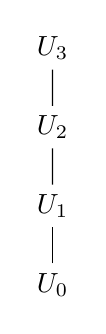
\begin{tikzpicture}
    \begin{scope}
      [level distance=1cm]
      \node{$\U_0$}[grow'=up]
      child {node {$\U_1$}
        child {node {$\U_2$}
          child {node {$\U_3$}}
        }
      };
    \end{scope}    
  \end{tikzpicture}
  % 
  \hfill
  %
  \begin{tikzpicture}
    \begin{scope}
      [level distance=1cm,
      level/.style={sibling distance=6cm/#1},
      nc/.style={gray}]
      \node{$T$}[grow'=up]
      child {node {$T_1$}
        child {node {$T_2$}
          child {node {$T_3$}}
          child {node {$T_3^{\sigma^4}$}}
        }
        child {node {$T_2^{\sigma^2}$}
          child[nc] foreach \l in {2,6} {node {$T_3^{\sigma^{\l}}$} edge from parent[dashed]}
        }
      }
      child {node {$T_1^\sigma$}
        child[nc] {node {$T_2^\sigma$} edge from parent[dashed]
          child[nc] foreach \l in {,5} {node {$T_3^{\sigma^{\l}}$} edge from parent[dashed]}
        }
        child[nc] {node {$T_2^{\sigma^3}$} edge from parent[dashed]
          child[nc] foreach \l in {3,7} {node {$T_3^{\sigma^{\l}}$} edge from parent[dashed]}
        }
      };
    \end{scope}
  \end{tikzpicture}
  
  \caption{The subproduct tree of $T$, in the case of a tower of
    quadratic extensions. Any generator of $\Gal(\U_3/\U_0)$ can be
    taken as $\sigma$. We gray out the nodes that the algorithm does
    not compute.}
  \label{fig:tree}
\end{figure}



Now we compute recursively the polynomials in $A_i\in\U_i[X]$ such
that $A_i(x)=y$. We start from $A_k=y$. Suppose $A_{i+1}$ is known,
then we apply the Chinese remainder algorithm of \cite[$\S$10.3]{vzGG}
to compute the polynomial $P\in\U_{i+1}[X]/T_i(X)$ such that
\begin{equation}
  \label{eq:crt}
  P \equiv A_{i+1}^\sigma \bmod T_{i+1}^\sigma
  \qquad\text{for any $\sigma\in\Gal(\U_{i+1}/\U_i)$.}
\end{equation}
It is clear that $P$ is invariant under $\Gal(\U_{i+1}/\U_i)$, hence
$P\in\U_i[X]/T_i(X)$ and by \eqref{eq:crt} it is evident that
$P(x)=A_{i+1}(x)=y$, thus $P=A_i$.

We have thus succeeded in interpolating $A=A_0$, without having to
build the whole subproduct tree. A similar algorithm was already given
in \cite{EnMo03}.


\paragraph{Back to our problem}
It is easy to realise that, on inputs $x(P)$ and $x(P')$, the
algorithm we just gave computes $A^{(0)}$. In fact, $T^{(0)}$ is
the minimal polynomial of $x(P)$ over $\F_q$ and $A^{(0)}$ is the
unique polynomial in $\F_q[X]/T^{(0)}(X)$ that satisfies
\eqref{eq:affine-minimal}.

This can be viewed as decomposing $\iota$ as the chain of
$\F_q$-linear isomorphisms
\begin{equation}
  \xymatrix{
    ^{\U_0[X_0]}/_{T_0(X_0)} \ar@{^{(}->}[r]^-{\iota_0} &
    \;\cdots\; \ar@{^{(}->}[r]^-{\iota_{k-1}} &
    ^{\U_k[X_k]}/_{T_k(X_k)} \ar@{^{(}->}[r]^-{\iota_k} &
    \U_k
  }
\end{equation}
defined by $\iota_k\circ\cdots\circ\iota_i(X_i) = x(P)$ for any $i$,
and then finding the preimage of $x(P')$ by inverting them one by
one.

Then, the Chinese remainder step we applied in \eqref{eq:crt} amounts
to invert $\iota_i$ by descending the lower path in the diagram below
\begin{equation}
  \xymatrix{
    ^{\U_i[X_i]}/_{T_i(X_i)} \ar@{^{(}->}[r]^-{\iota_i} \ar@{^{(}->}[d]^{\varepsilon} &
    ^{\U_{i+1}[X_{i+1}]}/_{T_{i+1}(X_{i+1})} \\
    ^{\U_{i+1}[Y]}/_{T_i(Y)} \ar@{^{(}->>}[r]^-{\gamma} &
    \bigoplus_\sigma {}^{\U_{i+1}[Y_{j}]}/_{\left(T_{i+1}\right)^\sigma(Y_{j})} \ar@{->>}[u]_{\pi}
  }
\end{equation}
where $\varepsilon$ is the canonical injection extending
$\U_i\subset\U_{i+1}$, $\gamma$ is the Chinese remainder isomorphism
and $\pi$ is projection onto the first coordinate.

Some care must be taken when $x(P)$ does not generate $\U_k$, but only
a subfield of index $2$. This happens when $c\not\in\F_q[c^2]$, and in
this case $\iota_0$ is not a field isomorphism. It is not to
difficult, however, to handle this case, as one only needs to take a
subgroup of index $2$ of $\Gal(\U_1/\U_0)$, instead of the whole
group, in the interpolation algorithm given above.

Observe that we could have used a different approach: after $T^{(0)}$
has been computed by \eqref{eq:minprod}, a polynomial $g\in\F_q[X]$
can efficiently be evaluated at $x(P)$ by successively lifting in
$\U_i$ and reducing modulo $T_i$ for $i=1,\ldots,k$. Thus, as noted
before, by the transposition principle we also have an efficient
algorithm to compute the power projection on $x(P)$; hence we can
apply \cite{PS06} to efficiently find $A^{(0)}$. However, this
approach cannot improve the overall complexity as it will be clear
in the next section.


\subsection{Complexity analysis}
\label{sec:C2-AS-FI:complexity}

The two algorithms for computing $T^{(0)}$ and $A^{(0)}$ are very
similar and run in parallel. We can merge them in one unique
algorithm.

We set some notation. Let $i_0$ be the largest index such that
$\U_{i_0} = \U_1$ and let $\frac{p-1}{2r} = [\F_q[c^2]:\F_q]$.  Remark
that all the $T^{(j)}$'s have degree $\frac{\euler(p^{k-i_0+1})}{2r}$.
At each level $i\ge i_0$, it does the following

\begin{enumerate}
\item for $\sigma \in \Gal(\U_{i+1}/\U_i)$, compute
  \begin{enumerate}
  \item\label{alg:T:gal} $\left(T_{i+1}\right)^\sigma$ and
  \item\label{alg:A:gal} $\left(A_{i+1}\right)^\sigma$ using
    \cite[\alg{IterFrobenius}]{DFS09},
  \end{enumerate}
\item\label{alg:T:prod} compute $T_i$ by \eqref{eq:minprod}
  through a subproduct tree as in \cite[Algo. 10.3]{vzGG},
\item\label{alg:A:CRA} compute $A_i$ by \eqref{eq:crt} through
  Chinese Reminder Algorithm \cite[Algo. 10.16]{vzGG},
\item\label{alg:T:push} convert $T_i$ and $A_i$ into
  elements of $\U_i[X]$ using \cite[\alg{Push-down}]{DFS09}.
\end{enumerate}

Steps \ref{alg:T:gal} and \ref{alg:A:gal} are identical. Both are
repeated $p$ times, each iteration taking $O\bigl(p^{k-i}{\sf
  L}(i-i_0)\bigr) \subset O\bigl({\sf L}(k-i_0)\bigr)$ by
\cite[Th. 17]{DFS09}.

Step \ref{alg:T:prod} takes $O\bigl(\Mult(p^{k-i_0+1}d/r)\log p\bigr)$
by \cite[Lemma 10.4]{vzGG} and step \ref{alg:A:CRA} has the same
complexity by \cite[Coro. 10.17]{vzGG}.

Step \ref{alg:T:push} takes $O\bigl(p^{k-i+1}{\sf L}(i-i_0)\bigr)
\subset O\bigl(p{\sf L}(k-i_0)\bigr)$.

When $i=0$ and $\U_1\ne\F_q$ the algorithm is identical but steps
\ref{alg:T:gal} and \ref{alg:A:gal} must be computed through a generic
Frobenius algorithm (using~\cite[Algorithm 5.2]{vzGS92}, for example)
and step \ref{alg:T:push} must use the implementation of $F_q[c]$ to
make the conversion (for example, linear algebra). In this case steps
\ref{alg:T:gal} and \ref{alg:A:gal} cost
$\Theta\bigl(\frac{p^{k-i_0}}{r}\ModComp(pd)\log d \bigr)$
by~\cite[Lemma 5.3]{vzGS92} and step \ref{alg:T:push} costs
$\Theta\bigl(p^{k-i_0}(pd)^2\bigr)$.

The total cost of the algorithm is then
\begin{equation*}
  \label{eq:T:complexity}
  O\left(\bigl(k-i_0\bigr)\bigl(p{\sf L}(k-i_0) + \Mult(p^{k-i_0+1}d/r)\log p\bigr) +
    \frac{p^{k-i_0}}{r}\bigl(\ModComp(pd)\log d + r(pd)^2\bigr) \right)
  \;\text{.}
\end{equation*}


\paragraph{The complete interpolation}
We compute all the $A^{(j)}$'s using this algorithm; there's
$p^{i_0-1}r$ of them. We then recombine them through a Chinese
remainder algorithm at a cost of $O\bigl(\Mult(p^kd)\log
p^{i_0-1}r\bigr)$. The total cost of the whole interpolation phase is
then
\begin{equation*}
  O\left(\bigl(k-i_0\bigr) \bigl(p{\sf L}(k) + \Mult(p^kd)\log p\bigr) +
    p^{k-1}\ModComp(pd)\log d + p^{k-1}r(pd)^2 + i_0\Mult(p^kd)\log p
  \right)
  \;\text{,}
\end{equation*}
that is
\begin{equation}
  \label{eq:interp}
  O\left(p{\sf L}(k)\log\left(\frac{\ell}{p^{i_0}}\right) + 
    \Mult(\ell d)\log\ell\log p +
    \frac{\ell}{p}\ModComp(pd)\log d +
    \ell (pd)^2
  \right)
  \;\text{.}
\end{equation}

Alternatively, once $A^{(0)}$ is known, one could compute the other
$A^{(j)}$'s using modular composition with the multiplication maps
of $E$ and $E'$ as suggested in \cite{Cou96}. However this approach
doesn't give a better asymptotic complexity because in the worst case
$A^{(0)}=A$. From a practical point of view, though, Brent's and
Kung's algorithm for modular composition \cite{BrKu78}, despite having
a worse asymptotic complexity, could perform faster for some set of
parameters. We will discuss this matter in Section
\ref{sec:C2-AS-FI-MC}.

If more than $\euler(p^k)/2$ points are needed, but less than
$\frac{p-1}{2}$, one can use the previous algorithm to interpolate
over the primitive $p^i$-torsion points for each $i=1,\ldots,k$. The
interpolating polynomials can then be recombined through a Chinese
remainder algorithm at a cost of $O\bigl(\Mult(p^kd)\log p^k\bigr)$,
which doesn't change the overall complexity of C2-AS-FI.


Putting together the complexity estimates of C2-AS and C2-AS-FI, we
have the following theorem.

\begin{theorem}
  \label{th:complexity}
  Assuming $\Mult(n) = n\log n\log\log n$, the algorithm C2-AS-FI has
  worst case complexity
  \begin{equation*}
    \tildO_{p,d,\log\ell}\left(
      p^2d^3 +
      \ModComp(p)pd +
      (pd)^\omega\log^2\ell +
      p^3\ell^2 d\log^3\ell + 
      p^2\ell^2 d^2+
      \left(\frac{\ell^2}{p} + p\right)\ModComp(pd)
    \right)
    \;\text{.}
  \end{equation*}
\end{theorem}



% Local Variables:
% mode:flyspell
% ispell-local-dictionary:"british"
% mode:TeX-PDF
% TeX-master: "ec-isogeny"
% End:
%
% LocalWords:  Schreier Artin pseudotrace Frobenius bivariate Joux Sirvent FFT
% LocalWords:  Couveignes isogenies Schoof isogeny cryptosystems Lercier moduli
% LocalWords:  precomputation arithmetics polylogarithmic Karatsuba embeddings
% LocalWords:  irreducibility

\section{The algorithm C2-AS-FI-MC}
\label{sec:C2-AS-FI-MC}

However asymptotically fast, the polynomial interpolation step is
quite expensive for reasonably sized data. Instead of repeating it
$\frac{\euler(p^k)}{2}$ times, one can use composition with the
Frobenius endomorphism $\frobisog_E$ in order to reduce the number of
interpolations in the final loop.

\subsection{The algorithm}
Suppose we have computed, by the algorithm of the previous Section,
the polynomial $T$ vanishing on the abscissae of $E[p^k]$ and an
interpolating polynomial $A_0\in\F_q[X]$ such that
\begin{equation*}
  A_0\bigl(x\bigl([n]P\bigr)\bigr) = x\bigl([n]P'\bigr)
  \quad\text{for any $n$.}
\end{equation*}
The group $\Gal(\U_k/\F_q) = \langle\frob\rangle$ acts on $E'[p^k]$
permuting its points and preserving the group structure. Thus, the
map (where polynomials act by evaluation) 
\begin{equation*}
  A_1 = A_0\circ\frob = \frob\circ A_0
\end{equation*}
is such that
\begin{equation*}
  A_1\bigl(x\bigl([n]P\bigr)\bigr) = x\bigl([n]\frobisog_{E'}(P')\bigr)
  \quad\text{for any $n$,}
\end{equation*}
where $\frobisog_{E'}$ is the Frobenius endomorphism of $E'$.  Since
$\frobisog_{E'}(P')$ is a generator of $E'[p^k]$, $A_1$ is one of the
polynomials that the algorithm C2 tries to identify to an isogeny. By
iterating this construction we obtain $[\U_k:\F_q]/2$ different
polynomials $A_i$ for the algorithm C2 with only one interpolation.

To compute the $A_i$'s, we first compute $F\in\F_q[X]$
\begin{equation}
  \label{eq:frob}
  F(X) = X^q \bmod T(X)
  \text{,}
\end{equation}
then for any $1\le i<[\U_k:\F_q]/2$
\begin{equation}
  \label{eq:modcomp}
  A_i(X) = A_{i-1}(X)\circ F(X) \bmod T(X)\text{.}
\end{equation}

If $\frac{\euler(p^k)}{[\U_k:\F_q]} = p^{i_0-1}r$, we must compute
$p^{i_0-1}r$ polynomial interpolations and apply this algorithm to
each of them in order to deduce all the polynomials needed by C2.


\subsection{Complexity analysis}
We compute \eqref{eq:frob} via square-and-multiply, this costs
$\Theta(d\Mult(p^kd)\log p)$ operations. Each application of
\eqref{eq:modcomp} is done via a \emph{modular composition}, the cost
is thus $O(\ModComp(p^k))$ operations in $\F_q$, that is
$O(\ModComp(p^k)\Mult(d))$ operations in $\F_p$. Using the algorithm
of~\cite{KeUm08} for modular composition, the complexity of
C2-AS-FI-MC wouldn't be essentially different from the one of
C2-AS-FI; however, in practice the fastest algorithm for modular
composition is~\cite{BrKu78}, and in particular the variant
in~\cite[Lemma 3]{KS98}, which has a worse asymptotic complexity, but
performs better on the instances we treat in
Section~\ref{sec:benchmarks}.

Notice that a similar approach could be used inside the polynomial
interpolation step (see Section \ref{sec:C2-AS-FI}) to deduce
$A_k^{(0)}$ from $A_0^{(0)}$ using modular composition with the
multiplication maps of $E$ and $E'$ as described in
\cite[$\S$2.3]{Cou96}. This variant, though, has an even worse
complexity because of the cost of computing multiplication maps.




% Local Variables:
% mode:flyspell
% ispell-local-dictionary:"british"
% mode:TeX-PDF
% TeX-master: "ec-isogeny"
% End:
%
% LocalWords:  Schreier Artin pseudotrace Frobenius bivariate Joux Sirvent FFT
% LocalWords:  Couveignes isogenies Schoof isogeny cryptosystems Lercier moduli
% LocalWords:  precomputation arithmetics polylogarithmic Karatsuba embeddings
% LocalWords:  irreducibility

\section{Smallest degree isogeny}
\label{sec:bounded}

We now present an extension to Couveignes algorithm that could be
useful in cryptographic application. It is well known that two curves
having the same number of points over a finite field are isogenous,
however this doesn't say anything on the degree of the isogeny
connecting them. Given two elliptic curves $E$ and $E'$ defined over
$\F_q$ and having the same number of points, we want to find the
smallest degree isogeny between them.

The simplest solution is to take any algorithm computing a fixed
degree isogeny and try all the degrees until an isogeny is found. If
$\ell$ is the degree of the smallest isogeny, this of course adds a
factor $\ell$ to the complexity of any polynomial time algorithm.

Couveignes' algorithm can be easily adapted to solve this problem at
no additional cost. We call this algorithm C2SD and we will only
discuss its most efficient variant C2SD-AS-FI.

Observe that, apart for the choice of $k$, the computation of $E[p^k]$
and the polynomial interpolation step do not depend at all on
$\ell$. The degree of the isogeny only comes into play in the last
part of the Cauchy interpolation, that is the rational function
reconstruction. We study more in detail this last step.


\paragraph{Rational Function Reconstruction}
Rational function reconstruction takes as input a degree $n$
polynomial $T$, a polynomial $A$ of degree less than $n$ and a target
degree $m\le n$ and outputs the unique rational function such that
\begin{equation*}
  A \equiv \frac{R}{V} \bmod T
\end{equation*}
and $\deg R < m$, $\deg V \le n-m$. This is done by computing a Bezout
relation $AV + TU = R$ with the expected degrees via an XGCD
algorithm. If a classical XGCD algorithm is used, one simply computes
all the lines
\begin{equation}
  \label{eq:XGCD}
  \begin{aligned}
    R_0 &= T, & U_0 &= 1, & V_0 &= 0,\\
    R_1 &= A, & U_1 &= 0, & V_1 &= 1,\\
    R_{i-1} &= Q_iR_i + R_{i+1}, & U_{i+1} &= U_{i-1}-Q_iU_i, & V_{i+1} &= V_{i-1}-Q_iV_i
  \end{aligned}
\end{equation}
and stops as soon as a remainder $R_{i+1}$ with $\deg R_{i+1}<m$ is
found. If a fast XGCD algorithm as \cite[Algo. 11.4]{vzGG} is used,
one directly aims at the two lines
\begin{equation}
  \label{eq:FastGCD}
  \begin{aligned}
    R_{h-2} &= Q_{h-1}R_{j-1} + R_h\\
    R_{h-1} &= Q_hR_h + R_{h+1}
  \end{aligned}
\end{equation}
such that $\deg R_{h+1} < m \le \deg R_h$ without computing the
intermediate lines.

When looking for an $\ell$-isogeny, one simply sets
$m=\ell+1$. Observe that if the algorithm doesn't return a rational
fraction $\frac{R}{V}$ with $\deg R = \ell$ and $\deg V = \ell -1 $,
then no such fraction congruent to $A$ modulo $T$ exists.

If $\ell$ is not \emph{a priori} known, we can still use the fact that
a separable isogeny with cyclic kernel must have $\deg R = \deg V +
1$. In fact if we suppose $R = R_i$ and $V = V_i$, then
\begin{align*}
  \deg T &= \deg V_{i+1} + \deg R_i,\\
  \deg R_i - \deg V_i &= \deg R_{i-1} - \deg V_{i+1}
\end{align*}
implies
\begin{equation*}
  \deg T + 1 = \deg R_{i-1} + \deg R_i  
  \;\text{.}
\end{equation*}
Hence, if $A$ is congruent to an $\ell$-isogeny with $\ell =
\left\lfloor\frac{\deg T}{2}\right\rfloor - t$ for some $t\ge0$, then
\begin{equation}
  \label{eq:degseq}
  \deg R_{i-1} =
  \left\lceil\frac{\deg T}{2}\right\rceil + t + 1 >
  \left\lfloor\frac{\deg T}{2}\right\rfloor - t = \deg R_i
  \;\text{.}
\end{equation}
Thus we can recover any isogeny having degree less than
$\left\lfloor\frac{\deg T}{2}\right\rfloor$ using either a classical
or a fast XGCD algorithm setting $m = \left\lceil\frac{\deg
    T}{2}\right\rceil + 1$.


\paragraph{Recognising an isogeny}
Once we have a rational fraction with the required degree, we have to
test if it really is an isogeny. In order to understand how often we
have to make this test, we introduce some more terminology. Let $n_i =
\deg R_i$, we call $(n_0,\ldots,n_r)$ the \emph{degree sequence} of
$A$ and $T$; a degree sequence is said \emph{normal} if $n_i = n_{i+1}
+ 1$ for any $i$.

\begin{proposition}
  \label{th:normseq}
  Let $f,g\in\F_q[X]$ be uniformly chosen random polynomials of
  respective degrees $n_0>n_1>0$ and let $(n_0, n_1, \ldots, n_r)$ be
  their degree sequence. For $0\le i < n_1$ define the binary random
  variables $X_i = 1 \Leftrightarrow i\in(n_0,n_1,\ldots,n_r)$, then
  the $X_i$ are independent random variables and $\mathrm{Prob}(X_i=0) =
  \frac{1}{q}$.
\end{proposition}
\begin{proof}
  Pairs of polynomials $f,g$ are in bijection with the GCD-sequence
  $(R_r, Q_r, \ldots, Q_1)$ constituted by their GCD and the quotients
  of the GCD algorithm. To each such sequence is associated a degree
  sequence
  \begin{equation*}
    (n_0,n_1,\ldots,n_r) =
    \left(\deg R_r + \sum_{i=1}^r\deg Q_i, \ldots, \deg R_r + \sum_{i=1}^1\deg Q_i, \deg R_r\right)
    \;\text{,} 
  \end{equation*}
  thus for any given degree sequence there are
  \begin{equation*}
    (q-1)q^{n_0-n_1}\cdot(q-1)q^{n_1-n_2}\cdot\cdots\cdot(q-1)q^{n_r} =
    (q-1)^{r+1}q^{n_0}
  \end{equation*}
  GCD-sequences.
 
  Let $I$ and $O$ be two disjoints subsets of $\{X_i\}$, the number of
  GCD-sequences such that $X\in I \Rightarrow X=1$ and $X\in O
  \Rightarrow X=0$,
  \begin{equation*}
     \sum_{s=0}^{n_1-\card{I}-\card{O}}\binom{n_1-\card{I}-\card{O}}{s}(q-1)^{s+2+\card{I}}q^{n_0} =
    (q-1)^{2+\card{I}}q^{n_0}q^{n_1-\card{I}-\card{O}}
    \;\text{.}
  \end{equation*}
  There are $(q-1)^2q^{n_0}q^{n_1}$ pairs of polynomials of degrees
  $n_0,n_1$, thus
  \begin{equation}
   \label{th:normseq:prob}
    \mathrm{Prob}\bigl(\{X = 1 \mid X\in I\},
    \{X=0\mid X\in O\}\bigr) = \left(\frac{q-1}{q}\right)^{\card{I}}\left(\frac{1}{q}\right)^{\card{O}}
    \;\text{.}
  \end{equation}
  The claim follows.
\end{proof}

Degree sequences associated to isogenies are in general not normal, in
fact if $\ell\le\left\lfloor\frac{\deg T}{2}\right\rfloor-t$, equation
\eqref{eq:degseq} shows that there must be at least a gap of degree
$2c$ in the degree sequence. Heuristically, we can expect that if the
polynomial $A$ doesn't correspond to an isogeny, then $A$ and $T$ act
like random polynomials, thus, by the proposition above, the
probability that $A$ looks like an isogeny of degree
$\ell\le\left\lfloor\frac{\deg T}{2}\right\rfloor-t$ is less than $\frac{1}{q^{2t}}$.

Therefore, by choosing an appropriate $t\in O(\log_q p^k)$, C2SD can
find any isogeny of degree less than $\frac{p^k-1}{4}-t$ at the same
cost of one run of C2. Also notice that C2SD is not restricted to
isogenies of degree prime to $p$ as it was already mentioned in
Section \ref{sec:C2:non-prime}.

No other method for computing isogenies is known to have a similar
generalisation, this makes C2SD-AS-FI interesting for practical
applications.




% Local Variables:
% mode:flyspell
% ispell-local-dictionary:"british"
% mode:TeX-PDF
% TeX-master: "ec-isogeny"
% End:
%
% LocalWords:  Schreier Artin pseudotrace frobenius bivariate Joux Sirvent FFT
% LocalWords:  Couveignes isogenies Schoof isogeny cryptosystems Lercier
% LocalWords:  precomputation arithmetics polylogarithmic Karatsuba precomputes
% LocalWords:  endomorphisms  isogenous

In this chapter we describe the implementations we made of the
algorithms of the previous chapter and some experimental results.

\section{Implementation of Couveignes' algorithm}
\label{sec:implementation}

We implemented \ctwoasfimc{} as \texttt{C++} programs using the
libraries \texttt{NTL}~\cite{shoup2003ntl} for finite field
arithmetics, \texttt{gf2x}~\cite{gf2x} for fast arithmetics in
characteristic $2$ and \texttt{FAAST} (see
Section~\ref{sec:artin-benchmarks}) for fast arithmetics in
Artin-Schreier towers.  We also have a Magma~\cite{MAGMA} prototype of
the same algorithm, not making use of the fast algorithms of
Chapter~\ref{cha:artin-schr-towers}.  This section mainly deals with
some tricks we implemented in order to speed up the computation.

\subsection{Building \texorpdfstring{$E[p^k]$}{E[pk]} and \texorpdfstring{$E'[p^k]$}{E[pk]}}
\label{sec:impl:torsion}

\paragraph{$p$-Torsion}
For $p\ne2$, \ctwo{} and its variants require to build the extension
$\F_q[c]$ where $c$ is a $(p-1)$-th root of $H_E$. In order to deal with
the lowest possible extension degree, it is a good idea to modify the
curve so that $[\F_q[c]:\F_q]$ is the smallest possible.

$[\F_q[c]:\F_q]$ is invariant under isomorphism, but taking a twist
can save us a quadratic extension. Let $u=c^{-2}$, the curve
\begin{equation*}
  \bar{E} : y^2 = x^3 + a_2ux^2 + a_4u^2x + a_6u^3
\end{equation*}
is defined over $\F_q[c^2]$ and is isomorphic to $E$ over $\F_q[c]$
via $(x,y)\mapsto(\sqrt{u}^2x,\sqrt{u}^3y)$. Its Hasse invariant is
$H_{\bar{E}} = (u)^{\frac{p-1}{2}}H_E = 1$, thus its $p$-torsion
points are defined over $\F_q[c^2]$.

In order to compute the $p^k$-torsion points of $E$ we build
$\F_q[c^2]$, we compute $\bar{P}$ a $p^k$-torsion points of $\bar{E}$
using $p$-descent, then we invert the isomorphism to compute the
abscissa of $P\in E[p^k]$. Since the Cauchy interpolation only needs
the abscissas of $E[p^k]$, this is enough to complete the
algorithm. Scalar multiples of $P$ can be computed without knowledge
of $y(P)$ using \hyperref[rk:montgomery]{Montgomery formulas}.

\pdfmcone{"Kummer surface" -> "Kummer variety".}  Remark that
for $p=2$ we use the same construction in an implicit way since we do
a $p$-descent on the Kummer variety.


\paragraph{$p^k$-Torsion points}
For $p\ne2$ we use Voloch's $p$-descent to compute the $p^k$-torsion
points iteratively as described in Section \ref{sec:C2}. To factor the
Artin-Schreier polynomial \eqref{th:voloch:cover}, we use the
algorithms from Section~\ref{sec:couveignes-algorithm} implemented in
\texttt{FAAST}.

To solve system \eqref{th:voloch:isom} we first compute
\begin{equation*}
  V(x,y) = \left(\frac{g(x)}{h^2(x)}, 
    sy\left(\frac{g(x)}{h^2(x)}\right)'\right)
\end{equation*}
through \titleref{sec:velu-formulas}.\footnote{Vélu formulas compute
  this isogeny up to an indeterminacy on the sign of the ordinate, the
  actual value of $s$ must be determined by composing $V$ with
  $\frobisog$ and verifying that it corresponds to $[p]$ by trying
  some random points.} Recall that we work on a curve having Hasse
invariant $1$, system \eqref{th:voloch:isom} can then be rewritten
\begin{equation*}
  \left\{
    \begin{aligned}
      \tilde{x}(P) &= \frac{g(x)}{h^2(x)}\\
      \tilde{y}(P) &= sy\left(\frac{g(x)}{h^2(x)}\right)'\\
      \tilde{z}(P) &= -2y\frac{h'(x)}{h(x)}
    \end{aligned}
  \right.
\end{equation*}
where $P$ is the point on the cover $C$ that we want to pull back
($\tilde{x}(P)$, $\tilde{y}(P)$ and $\tilde{z}(P)$ are just its
coordinates). After some substitutions this is equivalent to
\begin{equation*}
  \left\{
    \begin{aligned}
      \tilde{x}(P)h^2(x) - g(x) &= 0\\
      \left(\tilde{x}(P)h^2(x) - g(x) - \frac{\tilde{y}(P)}{s\tilde{x}(P)}h^2(x)\right)' &= 0
    \end{aligned}
  \right.
\end{equation*}
Then a solution in $x$ to this system is given by the GCD of the two
equations. Remark that proposition \ref{th:voloch} ensures there is
one unique solution. These formulas are slightly more efficient than
the ones in \cite[$\S$6.2]{lercier-algorithmique}.

For $p=2$ we use the library \texttt{FAAST} (for solving
Artin-Schreier equations) on top of \texttt{gf2x} (for better
performance). There is nothing special to remark about the
$2$-descent.


\subsection{Cauchy interpolation and loop}
\label{sec:impl:cauchy}
The polynomial interpolation step is done as described in Section
\ref{sec:C2-AS-FI}. As a result of this implementation, the polynomial
interpolation algorithm was added to the library \texttt{FAAST}.

The rational fraction reconstruction is implemented using a fast XGCD
algorithm on top of \texttt{NTL} and \texttt{gf2x}. This algorithm was
added to \texttt{FAAST} too.

The loop uses modular composition as in Section~\ref{sec:C2-AS-FI-MC}
in order to minimise the number of interpolations. The timings in the
next section clearly show that this non-asymptotically-optimal variant
performs much faster in practice.

To check that the rational fractions are isogenies we test their
degrees, that their denominator is a square and that they act as group
morphisms on a fixed number of random points. All these checks take a
negligible amount of time compared to the rest of the algorithm.


\subsection{Parallelisation of the loop}
\label{parallel}

The most expensive step of \ctwoasfimc{}, in theory as well as in
practice, is the final loop over the points of $E'[p^k]$. Fortunately,
this phase is very easy to parallelise with very little overhead.

Let $n$ be the number of processors we wish to parallelise on, suppose
that $[\U_k:\F_q]$ is maximal, then we make only one interpolation
followed by $\euler(p^k)/2$ modular compositions.\footnote{If
  $[\U_k:\F_q]$ is not maximal, the parallelisation is
  straightforward: we simply send one interpolation to each processor
  in turn.} We set $m=\left\lfloor\frac{\euler(p^k)}{2n}\right\rfloor$
and we compute the action of $\frobisog^{m}$ on $E[p^k]$ as in
Section~\ref{sec:C2-AS-FI-MC}:
\begin{equation*}
  F^{(m)}(X) = F(X) \circ \cdots \circ F(X) \bmod T(X)
  \;\text{,}
\end{equation*}
this can be done with $\Theta(\log m)$ modular compositions via a
binary square-and-multiply approach as in
Section~\ref{sec:modular-composition}.

Then we compute the $n$ polynomials
\begin{equation*}
  A_{mi}(X) = A_{m(i-1)}(X) \circ F^{(m)}(X) \bmod T(X)
\end{equation*}
and distribute them to the $n$ processors so that they each work on a
separate slice of the $A_i$'s. The only overhead is $\Theta(\log
(\ell/n))$ modular compositions with coefficients in $\F_q$, this is
acceptable in most cases.

\section{Implementation of \ctwoud{}}
\label{sec:implementation-c2-ud}
We modified our \texttt{C++} implementation of \ctwoasfimc{} to obtain
two variants of \ctwoud{}.

The first one takes an integer $k$ and looks for all isogenies of
degree $p^c\ell$ with $\ell$ prime to $p$, $\ell<\euler(p^k)/4$
and $c$ arbitrary. This is done by slightly modifying the modular
composition step of Section~\ref{sec:C2-AS-FI-MC}. Suppose we know an
interpolating polynomial $A_0$, that we view as a morphisms $E[p^k]\ra
E'[p^k]$ such that
\begin{equation}
  \label{eq:184}
  A_0\circ[n](P) = [n](P')
  \quad\text{for any $n$.}
\end{equation}
Then we compose with the Frobenius isogeny $\frobisog$
\begin{equation}
  \label{eq:185}
  A_1 \eqdef \frobisog\circ A_0:E[p^k]\ra {E'}^{(p)}[p^k]
  \text{,}
\end{equation}
where ${E'}^{(p)}$ is the curve
\begin{equation}
  \label{eq:186}
  E^{(p)}\;:\; y^2 = x^3+{a'}^px + {b}'^p
  \text{.}
\end{equation}
So $A_1$ is one of the polynomials that Couveignes algorithm computes
when looking for an isogeny between $E$ and ${E'}^{(p)}$. If $q=p^d$,
iterating $d$ times this construction, we fall back on $E'$, as we
would have if we had directly applied the
\hyperref[sec:curves-over-finite]{Frobenius automorphism} as in
Section~\ref{sec:C2-AS-FI-MC}. Thus, paying an additional factor of
$\log_p q$, we can compute any isogeny of degree $p^c\ell$ with
arbitrary $c$ and $\ell$ bounded as before.

When $\log_pq$ is large, the previous variant becomes unpractical. We
implemented a second variant using the algorithm described in
Section~\ref{sec:C2:non-prime}, this allows to compute any isogeny of
degree $\ell\le\euler(p^k)/4$, even if $p$ divides $\ell$. The
asymptotic cost of this variant is the same as one run of \ctwoasfimc{},
because the search for $\ell$ prime to $p$ dominates.



\section{Implementation of Lercier-Sirvent}
We implemented a Magma prototype of \titleref{alg:bmss}
and \titleref{alg:le-si}. In both cases we did
not take Remark~\ref{rk:bmss} into account, and only implemented the
variant using rational fraction reconstruction. We used Magma native
support for $p$-adics to construct the field $\Q_q$.

Both implementations differ from the description we gave in
Sections~\ref{sec:bmss} and~\ref{sec:lercier-sirvent} in that they
only take the degree $\ell$ and the equation of $E$ as input, and
compute an $\F_q$-isogenous curve, if it exists, by factoring the
modular polynomial in $\F_q[X]$.

\pdfmctwo{Atkin's MODULAR polynomial. Not "canonical".}
Instead of the classical modular polynomials $\Modpol_\ell$ we used
Atkin's modular polynomials $\Modpol^\ast_\ell$ since they have
smaller coefficients and degree; this does not change the other steps
of the algorithm.

The modular polynomials were not computed on the fly as suggested in
Section~\ref{sec:lercier-sirvent}, instead they were taken from the
tables precomputed in Magma. This implies that the implementation has
an asymptotic complexity cubic in $\ell$, however we will see that
even this implementation behaves well in practice.


% Local Variables:
% mode:flyspell
% ispell-local-dictionary:"american"
% mode:TeX-PDF
% TeX-master: "../these"
% mode:reftex
% End:
%
% LocalWords:  Schreier Artin pseudotrace Frobenius bivariate Joux Sirvent FFT
% LocalWords:  Couveignes isogenies Schoof isogeny cryptosystems Lercier Hasse
% LocalWords:  precomputation arithmetics polylogarithmic Karatsuba precomputes
% LocalWords:  endomorphisms 

\section{Benchmarks}
\label{sec:benchmarks}
We ran various experiments to compare the different variants of the
algorithm \ctwo{} between themselves and to \titleref{alg:le-si}. All
the experiments were run on four dual-core Intel Xeon E5520 (2.26GHz),
using the parallelized version of the algorithm in some cases. Magma
2.16 was used to run Magma experiments.

\paragraph{Magma vs. \texttt{FAAST}}
\label{sec:magma-vs.-textttf}
The first set of experiments was run to evaluate the benefits of using
the algorithms of Chapter~\ref{cha:artin-schr-towers}. We selected
pairs of isogenous curves over $\F_{2^{101}}$ such that the height of
the tower is maximal (observe that this is always the case for
cryptographic curves).  We compared the Magma prototype to the
\texttt{FAAST}-based implementation of \ctwoasfimc{} using the
\texttt{zz\_p} and \texttt{GF2} data types (see
Section~\ref{sec:artin-benchmarks}).

\begin{figure}
  \centering
  \includegraphics[width=0.9\textwidth]{isogeny/p2}
  \caption{Comparative timings for different implementations of \ctwoasfimc{} with curves defined over $\F_{2^{101}}$. Plot in logarithmic scale.}
  \label{fig:2-101}
\end{figure}

The results are in figure~\ref{fig:2-101}: we plot a line for the
average running time of the algorithm and bars around it for minimum
and maximum execution times of the final loop. Besides the dramatic
speedup obtained by using the ad-hoc type \texttt{GF2}, the
algorithmic improvements of \texttt{FAAST} over Magma are evident as
even \texttt{zz\_p} is one order of magnitude faster.

\begin{table}
  \centering
  \begin{tabular}{r r r r r r r r}
    \hline
    $\ell$ & $E[p^k]$ & $E'[p^k]$ & FI & RFR & MC & Avg tries & Avg loop time\\
    \hline
    31  &  0.3529 &  0.3529 & 0.3569 & 0.00125 & 0.00055 &  32 &   0.058\\
    61  &  0.9848 &  0.9848 & 0.8268 & 0.00343 & 0.00228 &  64 &   0.365\\
    127 &  2.6636 &  2.6626 & 1.8927 & 0.01090 & 0.00872 & 128 &   2.511\\
    251 &  6.9809 &  6.9779 & 4.2833 & 0.03092 & 0.03494 & 256 &  16.860\\
    397 & 18.1052 & 18.0952 & 9.7385 & 0.07325 & 0.14117 & 512 & 109.783\\
  \end{tabular}
  \caption{Comparative timings for the phases of \ctwoasfimc{} for curves over $\F_{2^{101}}$.}
  \label{tab:C2}
\end{table}

Table~\ref{tab:C2} shows detailed timings for each phase of
\ctwoasfimc{}. The column FI reports the time for one interpolation, the
column MC the time for one modular composition; comparing these two
columns the gain from passing from \ctwoasfi{} to \ctwoasfimc{} is
evident. Columns RFR (rational fraction reconstruction) and MC
constitute the Cauchy interpolation step that is repeated in the final
loop. The last column reports the average time spent in the loop: it
is by far the most expensive phase and this justifies the attention we
paid to FI and MC; only on some huge examples we approached the
crosspoint between these two algorithms.


\paragraph{\ctwoud{}}
\label{sec:c2-ud}
Next we ran experiments on \ctwoud{}. The first observation was that the
heuristic argument --on the probability that a degree sequence not
associated to an isogeny is not normal-- is well verified in practice:
except for a degree $2$ symmetry verified in characteristic $2$,
polynomials not associated to an isogeny very rarely gave a degree
sequence with a gap around the middle.

\pdfmcone{Added some blabla on Teske's cryptosystem.}
Looking for isogenies of unknown degree may be of some cryptographic
significance. For example, Teske's trapdoor cryptosystem selects a
binary field of composite degree ($\F_{2^{7\cdot 23}}$, in the
proposal) and chooses an elliptic curve $E$ vulnerable to the GHS
attack~\cite{gaudry+hess+smart02}. Then hides $E$ by taking a random
path of isogenies of small degrees landing on a curve $E'$ not
vulnerable to GHS, and uses $E'$ as public key. The security of the
cryptosystem comes from the assumption that it is infeasible to find a
GHS-vulnerable curve isogenous to $E'$, without the knowledge of the
isogeny path. 

The \emph{trapdoor} of the cryptosystem is the curve $E$: it is given
to a trusted authority so that --using an isogeny path from $E'$ to
$E$ and a GHS attack-- it has the power of deciphering messages at a
relatively high computational cost. This feature rests on the
assumption that it is feasible, but relatively hard, to compute any
isogeny path from $E$ to $E'$.

In this context, it may be interesting to verify that $E$ and $E'$ are
not related by an isogeny of too low degree.
From~\cite[Appendix~A]{teske06}, we took the two curves defined over
$F_{2^{161}}=\F_2[z]/(z^{161}+z^{18}+1)$ of $j$ invariants:

$1/j = z^{152} + z^{143} + z^{139} + z^{136} + z^{135} + z^{133} +
z^{130} + z^{125} + z^{124} + z^{122} + z^{120} + z^{119} + z^{118} +
z^{117} + z^{116} + z^{114} + z^{113} + z^{112} + z^{110} + z^{109} +
z^{106} + z^{105} + z^{103} + z^{102} + z^{101} + z^{99} + z^{97} +
z^{96} + z^{92} + z^{91} + z^{88} + z^{87} + z^{86} + z^{85} + z^{81}
+ z^{78} + z^{77} + z^{76} + z^{75} + z^{73} + z^{71} + z^{69} +
z^{68} + z^{67} + z^{66} + z^{63} + z^{59} + z^{58} + z^{53} + z^{51}
+ z^{50} + z^{49} + z^{48} + z^{46} + z^{45} + z^{44} + z^{42} +
z^{38} + z^{34} + z^{3} + z^{32} + z^{31} + z^{29} + z^{27} + z^{26} +
z^{24} + z^{23} + z^{22} + z^{21} + z^{20} + z^{19} + z^{18} + z^{17}
+ z^{16} + z^{15} + z^{14} + z^{13} + z^{12} + z^{10} + z^{7} + z^{6}
+ z^{4} + z^{3} + z^{2}$,

$1/j'=z^{160} + z^{156} + z^{155} + z^{153} +z^{152} +z^{151} +z^{150}
+z^{149} +z^{148} +z^{147} +z^{146} +z^{145} +z^{143} +z^{142}
+z^{141} +z^{130} +z^{129} + z^{127} + z^{126} + z^{125} + z^{124} +
z^{123} + z^{120} + z^{118} + z^{112} + z^{109} + z^{104} + z^{103} +
z^{102} + z^{101} + z^{99} + z^{98} +z^{97} +z^{96} +z^{93} +z^{92}
+z^{91} +z^{90} +z^{88} +z^{85} +z^{83} +z^{77} +z^{74} +z^{70}
+z^{68} +z^{65} +z^{64} +z^{63} + z^{62} + z^{61} + z^{60} + z^{58} +
z^{57} + z^{55} + z^{50} + z^{48} + z^{45} + z^{41} + z^{38} + z^{37}
+ z^{36} + z^{33} + z^{31} + z^{30} + z^{27} +z^{26} +z^{24} +z^{23}
+z^{22} +z^{21} +z^{20} +z^{19} +z^{17} +z^{16} +z^{14} +z^{13}
+z^{10} +z^{8} +z^{7} +z^{4} +z^{3} +z$.

We ran our two variants of \ctwoud{} on the two curves to certify the
conjectured property that no unexpected isogeny of low degree exists
between the two curves.

In 258 cpu-hours we were able to prove that no isogeny of degree
$p^c\ell$ for $\ell<2^{11}$ and $c$ arbitrary exists between the two
curves; in 694 cpu-hours we were able to prove that no isogeny of
degree less than $2^{13}$ exists either. We stress the fact that,
albeit of little interest, this computation would have been impossible
without the (surprising) discovery of \ctwoud{}.


\paragraph{Couveignes vs. Lercier-Sirvent}
Finally, we ran experiments on
\titleref{alg:le-si}. 
Table~\ref{tab:ls} shows
timings for the different phases of the algorithm for some isogeny
degrees. The first column is the time spent to find a root of
$\Modpol_\ell(X,j_E)$ in $\F_q$, the second column summarizes the time
spent to lift this root in $\Q_q$ and apply Elkies'
formulas. DiffSolve is the time spent solving the differential
equation, it is clearly the most expensive phase, although not the
most important asymptotically. RFR is the time for rational fraction
reconstruction, its rapid growth is justified by the fact that we
implemented it on top of a quadratic XGCD algorithm.

\begin{table}
  \pdfmcthree{This table has changed.}
  \centering
  \begin{tabular}{r r r r}
    \hline
    $\ell$ & Lift & DiffSolve & RFR\\
    \hline
    31  &   0.570 &   14.830 & 0.010\\
    103 &   5.160 &  274.550 & 0.250\\
    149 &  12.510 &  815.320 & 0.590\\
    239 &  21.420 & 1470.240 & 1.950\\
    331 & 113.500 & 4204.610 & 4.890\\
    389 & 147.340 & 5166.730 & 7.360\\
  \end{tabular}
  \caption{Comparative timings for the phases of \titleref{alg:le-si} 
    for curves over $\F_{3^{64}}$.}
  \label{tab:ls}
\end{table}


\begin{figure}
  \centering
  \includegraphics[height=0.45\textwidth]{isogeny/C2-LS}
  \includegraphics[height=0.45\textwidth]{isogeny/C2-LS2}
  \caption{Comparative timings for \ctwoasfimc{} (C2) and
    \titleref{alg:le-si} (LS) over different curves. Plot in
    logarithmic scale.}
  \label{fig:comp}
\end{figure}

We also compared the running times of \ctwoasfimc{} and
\titleref{alg:le-si} over curves of half the cryptographic size in
figure~\ref{fig:comp} (left) and five times the cryptographic size in
figure~\ref{fig:comp} (right). We only plot average times for \ctwo{},
in characteristic $2$ we only plot the timings for \texttt{GF2}. From
the plot it is clear that \ctwoasfimc{} only performs better than
\titleref{alg:le-si} for $p=2$, but in this case Lercier's
algorithm~\cite{lercier96} is much faster.  Contradicting theory, the
asymptotic behavior of \titleref{alg:le-si} looks worse than the one
of \ctwoasfimc{}; however comparing a Magma prototype to our highly
optimized implementation of \ctwoasfimc{} is somewhat unfair.

Furthermore, it is unlikely that \ctwoasfimc{} could be practical for
any $p>3$ because of its high dependence on $p$, while
\titleref{alg:le-si} scales pretty well with the characteristic as
shown in figure~\ref{fig:LSp}.

Considering that the asymptotic dependency of Couveignes' algorithm in
$\log q$ and in $p$ is worse than the one of \titleref{alg:le-si}
(compare Eq.~\eqref{eq:interp} to
Proposition~\ref{th:lercier-sirvent}), there are very few regions
where Couveignes' algorithm stays of practical or theoretical
interest.

\pdfmcone{People don't like pessimism.}  Ironically, the
techniques presented in this document were developed in view of an
efficient implementation of Couveignes' algorithm, but, for the
moment, their only practical application seems to be \ctwoud{}. Our hope
is that other interesting applications may be found in the future.

\begin{figure}
  \centering
  \includegraphics[width=0.9\textwidth]{isogeny/LSp}
  \caption{Timings for \titleref{alg:le-si} for different fields. We
    increase $p$ while keeping constant $d$ and the isogeny degree.}
  \label{fig:LSp}
\end{figure}


% Local Variables:
% mode:flyspell
% ispell-local-dictionary:"american"
% TeX-master: "../these"
% mode: TeX-PDF
% mode:reftex
% End:
%
% LocalWords:  Schreier Artin pseudotrace Frobenius bivariate Joux Sirvent FFT
% LocalWords:  Couveignes isogenies Schoof isogeny cryptosystems Lercier
% LocalWords:  precomputation arithmetics polylogarithmic Karatsuba precomputes
% LocalWords:  endomorphisms  isogenous


% Local Variables:
% mode:flyspell
% ispell-local-dictionary:"american"
% mode:TeX-PDF
% mode:reftex
% End:
%

